\renewcommand{\thesubfigure}{\alph{subfigure}}
\renewcommand{\figurename}{Figure}
\renewcommand{\tablename}{Table}
\setcounter{figure}{0}
\setcounter{table}{0}
\setcounter{equation}{0}	% Reset equation numbering https://tex.stackexchange.com/questions/207532/reset-equation-numbering-after-each-section

\chapter*{Synopsis}
\addcontentsline{toc}{chapter}{Synopsis} 

\paragraph*{Relevance of the chosen topic.}
\paragraph*{Goal.}
\paragraph*{Objectives.}
\paragraph*{Research methods.}
\paragraph*{Assertions that are presented for defense.}
\paragraph*{The novelty of research.}
\paragraph*{The scientific and technical objective.}
\paragraph*{The research object.}
\paragraph*{The research subject.}
\paragraph*{The theoretical significance.}
\paragraph*{The practical significance.}
\paragraph*{The accuracy of the obtained results.}

\paragraph*{Implementation of research results.}
\paragraph*{Approbation of research results.}
The main results of the thesis were presented at the following conferences:
\printConferenceEN
\paragraph*{Personal contribution of the author.}
\paragraph*{Thesis structure and number of pages.}

\newpage
\section*{Main contents of the work}

In Chapter~\ref{ch:ch1}...
\begin{center}
	General thesis summary
\end{center}
\begin{figure}
	\centering
	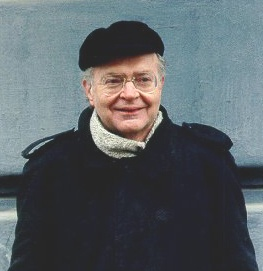
\includegraphics[width=0.4\linewidth]{images/knuth}
	\caption{Knuth}
	%\label{fig:my_label2}
\end{figure}
\begin{table}
	\centering
	\captionsetup{justification=centering} % выравнивание подписи по-центру
	\caption{Basic SI quantities}%\label{tab:unit:base}
	\begin{tabular}{llc}
		\toprule
		Name 	& 	Command 	& 	Symbol         \\
		\midrule
		Ampere     & \verb|\ampere| & \si{\ampere}   \\
		Candela   & \verb|\candela| & \si{\candela}  \\
		\bottomrule
	\end{tabular}
\end{table}

\begin{align} %\label{eq:sec1}
	1+2=3
\end{align}

\begin{assumption-syn-en}
	Here and below, the sign of the coefficient when controlling $b_m$
	accepted as known. Without loss of generality, we assume $b_m >0$.
\end{assumption-syn-en}
\begin{lemma-syn-en} \label{lemma1:1}
	content...
\end{lemma-syn-en}

\begin{proof}[Proof Lemma \ref{lemma1:1}]
	content...
\end{proof}

\section*{Publications relevant to this thesis}
Key results of research are described in \theAllMyPapers~publications. Among them \theScopusPapers~are published in a journal indexed by Scopus and Web of Science. 
%and 0 published in journals recommended by the Higher Attestation Commission (VAK) 
%and 1 is published in other sources. One certificate of state registration of a computer program has also been obtained.\\

Publications in international journals indexed by Scopus and Web of Science:
\printPapperScopus

Publications indexed in Russian journal included in the List of the Higher Attestation Commission: 
%\printPapperVak

Publications in other journals:
\printPapperOther
